
\section{HU3 Pantalla de visualización}

Se muestra en pantalla los datos de los alumnos, con los campos de “Num. Lista”, “Matrícula”, “Nombre(s) Apellido(s)” y “Selección”; el primero muestra el número de lista asignado, el siguiente la matrícula con la cual se identifica al alumno, el tercero su nombre junto con su apellido, y la selección que se llevará a cabo mediante cuadros de selección. 
Este último servirá para hacer una selección múltiple al momento de eliminar\\
Sin embargo al momento de actualizar el alumno, basta con seleccionar un registro y este se copiará a las cajas de texto para su edición \\
El botón de “Eliminar” nos mostrará una ventana emergente con los datos del alumno.
Existe una entrada de texto el cual servirá para buscar a un alumno por su nombre y apellido, cuenta con la leyenda: “Búsqueda de alumno . . .”. Esto tiene como fin hacer la búsqueda del alumno más fácil cuando se tiene un gran número de alumnos.

\begin{figure}[h]
	\centering
	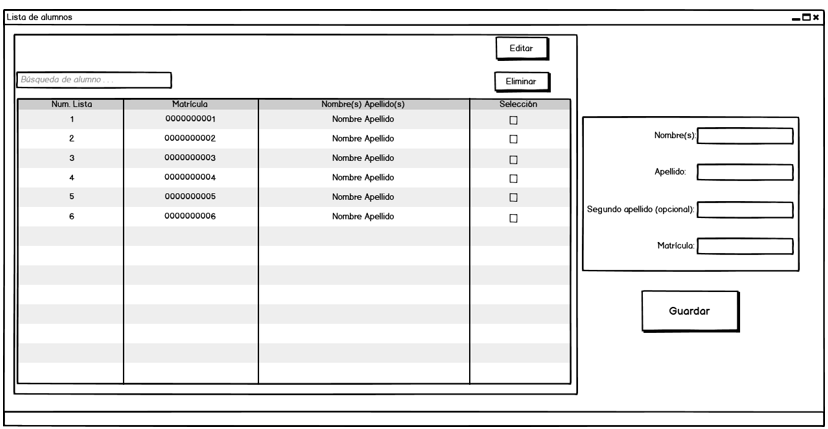
\includegraphics[scale=0.5]{./HistoriasUsuario/imagenes/IHU6.png}
	\caption{Pantalla de visualización}
\end{figure}
